
%(BEGIN_QUESTION)
% Copyright 2009, Tony R. Kuphaldt, released under the Creative Commons Attribution License (v 1.0)
% This means you may do almost anything with this work of mine, so long as you give me proper credit

Read and outline the ``Bernoulli's Equation'' subsection of the ``Fluid Mechanics'' section of the ``Physics'' chapter in your {\it Lessons In Industrial Instrumentation} textbook.  Note the page numbers where important illustrations, photographs, equations, tables, and other relevant details are found.  Prepare to thoughtfully discuss with your instructor and classmates the concepts and examples explored in this reading.

\underbar{file i04035}
%(END_QUESTION)





%(BEGIN_ANSWER)


%(END_ANSWER)





%(BEGIN_NOTES)

If the flow of fluid through a pipe is inviscid (free of viscous forces dissipating energy via friction) and there is no pump or valve or other energy-translating device placed in the stream, we may safely assume the energy of that fluid remains constant at it travels through different portions of the piping system.  This is a consequence of the Law of Energy Conservation, and is expressed in Bernoulli's equation which specifies the total energy in a fluid stream in three ``heads'' (elevation, velocity, and pressure):

$$z_1 \rho g + {v_1^2 \rho \over 2} + P_1 = z_2 \rho g + {v_2^2 \rho \over 2} + P_2$$

$$z_1 + {v_1^2 \over {2 g}} + {P_1 \over \gamma} = z_2 + {v_2^2 \over {2 g}} + {P_2 \over \gamma}$$

\noindent
Where,

$z$ = Height of fluid (from a common reference point, usually ground level)

$\rho$ = Mass density of fluid

$\gamma$ = Weight density of fluid ($\gamma = \rho g$)

$g$ = Acceleration of gravity

$v$ = Velocity of fluid

$P$ = Pressure of fluid

\vskip 10pt

Potential energy in the form of liquid elevation above ground level ($z \rho g$) is analogous to potential energy of a raised mass ($mgh$).  Kinetic energy in the form of liquid velocity ($\rho v^2 \over 2$) is analagous to kinetic energy of a moving mass (${1 \over 2} mv^2$).  Potential energy of a fluid expressed as a {\it pressure} ($P$) has no direct analogue in the world of solids.

\vskip 10pt

It is critically important that all units are kept consistent when applying Bernoulli's equation to real flow applications.  If velocity is expressed in feet per second, then pressure must be expressed in pounds per square feet, gravity in feet per second squared, and density in slugs per cubic foot.

\vskip 10pt

The relationship between weight density ($\gamma$) and mass density ($\rho$) is given by the following formula:

$$\gamma = \rho g$$

$g$ is the acceleration of Earth's gravity expressed as 32.2 feet per second squared, or 9.81 meters per second squared.

\vskip 10pt

A good problem-solving approach to use for heavily mathematical problems is to write all relevant formulae, then circle those variables you happen to know the values of as well as identify those variables that are (yet) unknown to you, tying in other formulae as necessary to quantify those unknowns.










\vskip 20pt \vbox{\hrule \hbox{\strut \vrule{} {\bf Suggestions for Socratic discussion} \vrule} \hrule}

\begin{itemize}
\item{} {\bf Describe the problem-solving strategy used in solving the example problem in this subsection of the book, and explain how this strategy may be applied in a general sense to any physics problem.}
\item{} Explain {\it why} Bernoilli's equation is true; i.e. what fundamental principle of nature is reflected in this equation.
\item{} Identify a practical application where we could {\it not} apply Bernoulli's equation to two different points in a piping system.
\item{} Explain the function of an {\it ejector} (gas flow) or an {\it eductor} (liquid flow).
\item{} Explain why an {\it eductor} is used to draw chlorine gas into wastewater for disinfection of that water, rather than inject pressurized chlorine to do the same.
\end{itemize}














\vfil \eject

\noindent
{\bf Summary Quiz:}

Choose the statement most accurately describing the relationship between the pressure gauges' readings in this liquid piping system, based on Bernoulli's equation.  Assume a constant rate of flow in the direction shown:

$$\includegraphics[width=15.5cm]{i04035x01.eps}$$

$$z_1 \rho g + {v_1^2 \rho \over 2} + P_1 = z_2 \rho g + {v_2^2 \rho \over 2} + P_2$$

\begin{itemize}
\item{} Gauge 3 reads less pressure than Gauge 1
\vskip 5pt 
\item{} Gauge 3 reads more pressure than Gauge 1
\vskip 5pt 
\item{} Gauge 1 reads less pressure than Gauge 2
\vskip 5pt 
\item{} Gauge 3 reads more pressure than Gauge 2
\end{itemize}


%INDEX% Reading assignment: Lessons In Industrial Instrumentation, Fluid Mechanics (Bernoulli's Equation)

%(END_NOTES)


